%%%%%%%%%%%%%%%%%%%%%%%%%%%%%%%%%%%%%%%%%%%%%%%%%%%%%%%%%%%%%%%%%%%%%%%%%%%%%%%
% intro.tex: Introduction to the thesis
%%%%%%%%%%%%%%%%%%%%%%%%%%%%%%%%%%%%%%%%%%%%%%%%%%%%%%%%%%%%%%%%%%%%%%%%%%%%%%%%
\chapter{Introduction}
\label{intro_chapter}
%%%%%%%%%%%%%%%%%%%%%%%%%%%%%%%%%%%%%%%%%%%%%%%%%%%%%%%%%%%%%%%%%%%%%%%%%%%%%%%%

\section{Introduction}

%%In order to meet the increasing requirements, many modern combustors involve high-pressure working environments. For rocket engines, to achieve high specific impulse and thrust, combustion chamber pressure $P_{cc}$ is elevated for many rocket engines. For example, the space shuttle main engine (SSME) has a chamber pressure $P_{cc}$ = 19 MPa, RD-170 $P_{cc}$ = 25 MPa, and Vulcain 2 engine $P_{cc}$ = 11.5 MPa \cite{arnold2009circumferential}.
%An enhencement of the specific impulse and thrust are the main objectives for next-generation rocket propulsion systems. Because the combustion chamber pressure is the driving parameter for engine size, these ambitious goals can only be realized with higher combustion chamber pressure. The . A higher combustion pressure pcc is used for many roket engine. for example  space shuttle main engine (SSME) pcc = 19 MPa [4], RD-170 pcc= 25 MPa, e European Ariane 5 first-stage Vulcain 2 engine pcc  11:5 MPa. \cite{arnold2009circumferential}
%%For next-generation gas turbines, higher working pressure is used to obatin a higher thermal efficiency. Fig.~\ref{Intro_gas_turbine} shows the combustor pressure is increasing, and the pressure of some gas turbines is even higher than the critical pressure of the air and fuel in recent years. In addition, high pressure is also required by new designs to achieve other advantages. For example, in semi-closed supercritical \ce{CO2} gas turbine systems, the heat input typically comes from oxy-fuel combustion in supercritical \ce{CO2}. Besides higher efficiency, this power cycle is one of the potential solutions to effectively remove \ce{CO2} and \ce{NO_x} emissions from power generation.

To meet the escalating demands of modern applications, a multitude of modern combustor designs operate within high-pressure environments. This shift is notably exemplified in rocket engines, where the augmentation of combustion chamber pressure, denoted as $P_{cc}$, is pivotal for attaining superior specific impulse and thrust. For instance, the Space Shuttle Main Engine (SSME) achieves a chamber pressure of $P_{cc}$ = 19 MPa, the RD-170 rockets soar at $P_{cc}$ = 25 MPa, and the Vulcain 2 engine achieves $P_{cc}$ = 11.5 MPa \cite{arnold2009circumferential}. Furthermore, the next-generation gas turbines harness elevated working pressures to optimize thermal efficiency, as depicted in Fig.~\ref{Intro_gas_turbine}, where combustor pressures steadily ascend. In recent years, the pressure levels of certain gas turbines have exceeded even the critical pressure of the air and fuel. This escalating pressure requirement is not only driven by the pursuit of heightened efficiency but also by the pursuit of other operational advantages. A notable example of such advancements can be found in semi-closed supercritical CO2 gas turbine systems. Here, the primary heat input stems from oxy-fuel combustion within a supercritical CO2 medium. Beyond the evident efficiency gains, this power cycle presents itself as a promising solution for the effective mitigation of CO2 and NOx emissions in power generation. Furthermore, it's worth noting that diesel engines operate within a pressure range of 10 to 30 bar \cite{jofre2021transcritical}, which places them in a similar high-pressure realm, often approaching or exceeding the critical pressure of both air and liquid fuel.
%%Morevoer, diesel engines operate within the range of 10 to 30 bar \cite{jofre2021transcritical}. These high working pressures are also comparable to or even higher than the critical pressure of air and liquid fuel.

\begin{figure}[htb]
    \centering
    \subfigure{
        %\begin{minipage}[t]{0.5\linewidth}
        \centering
        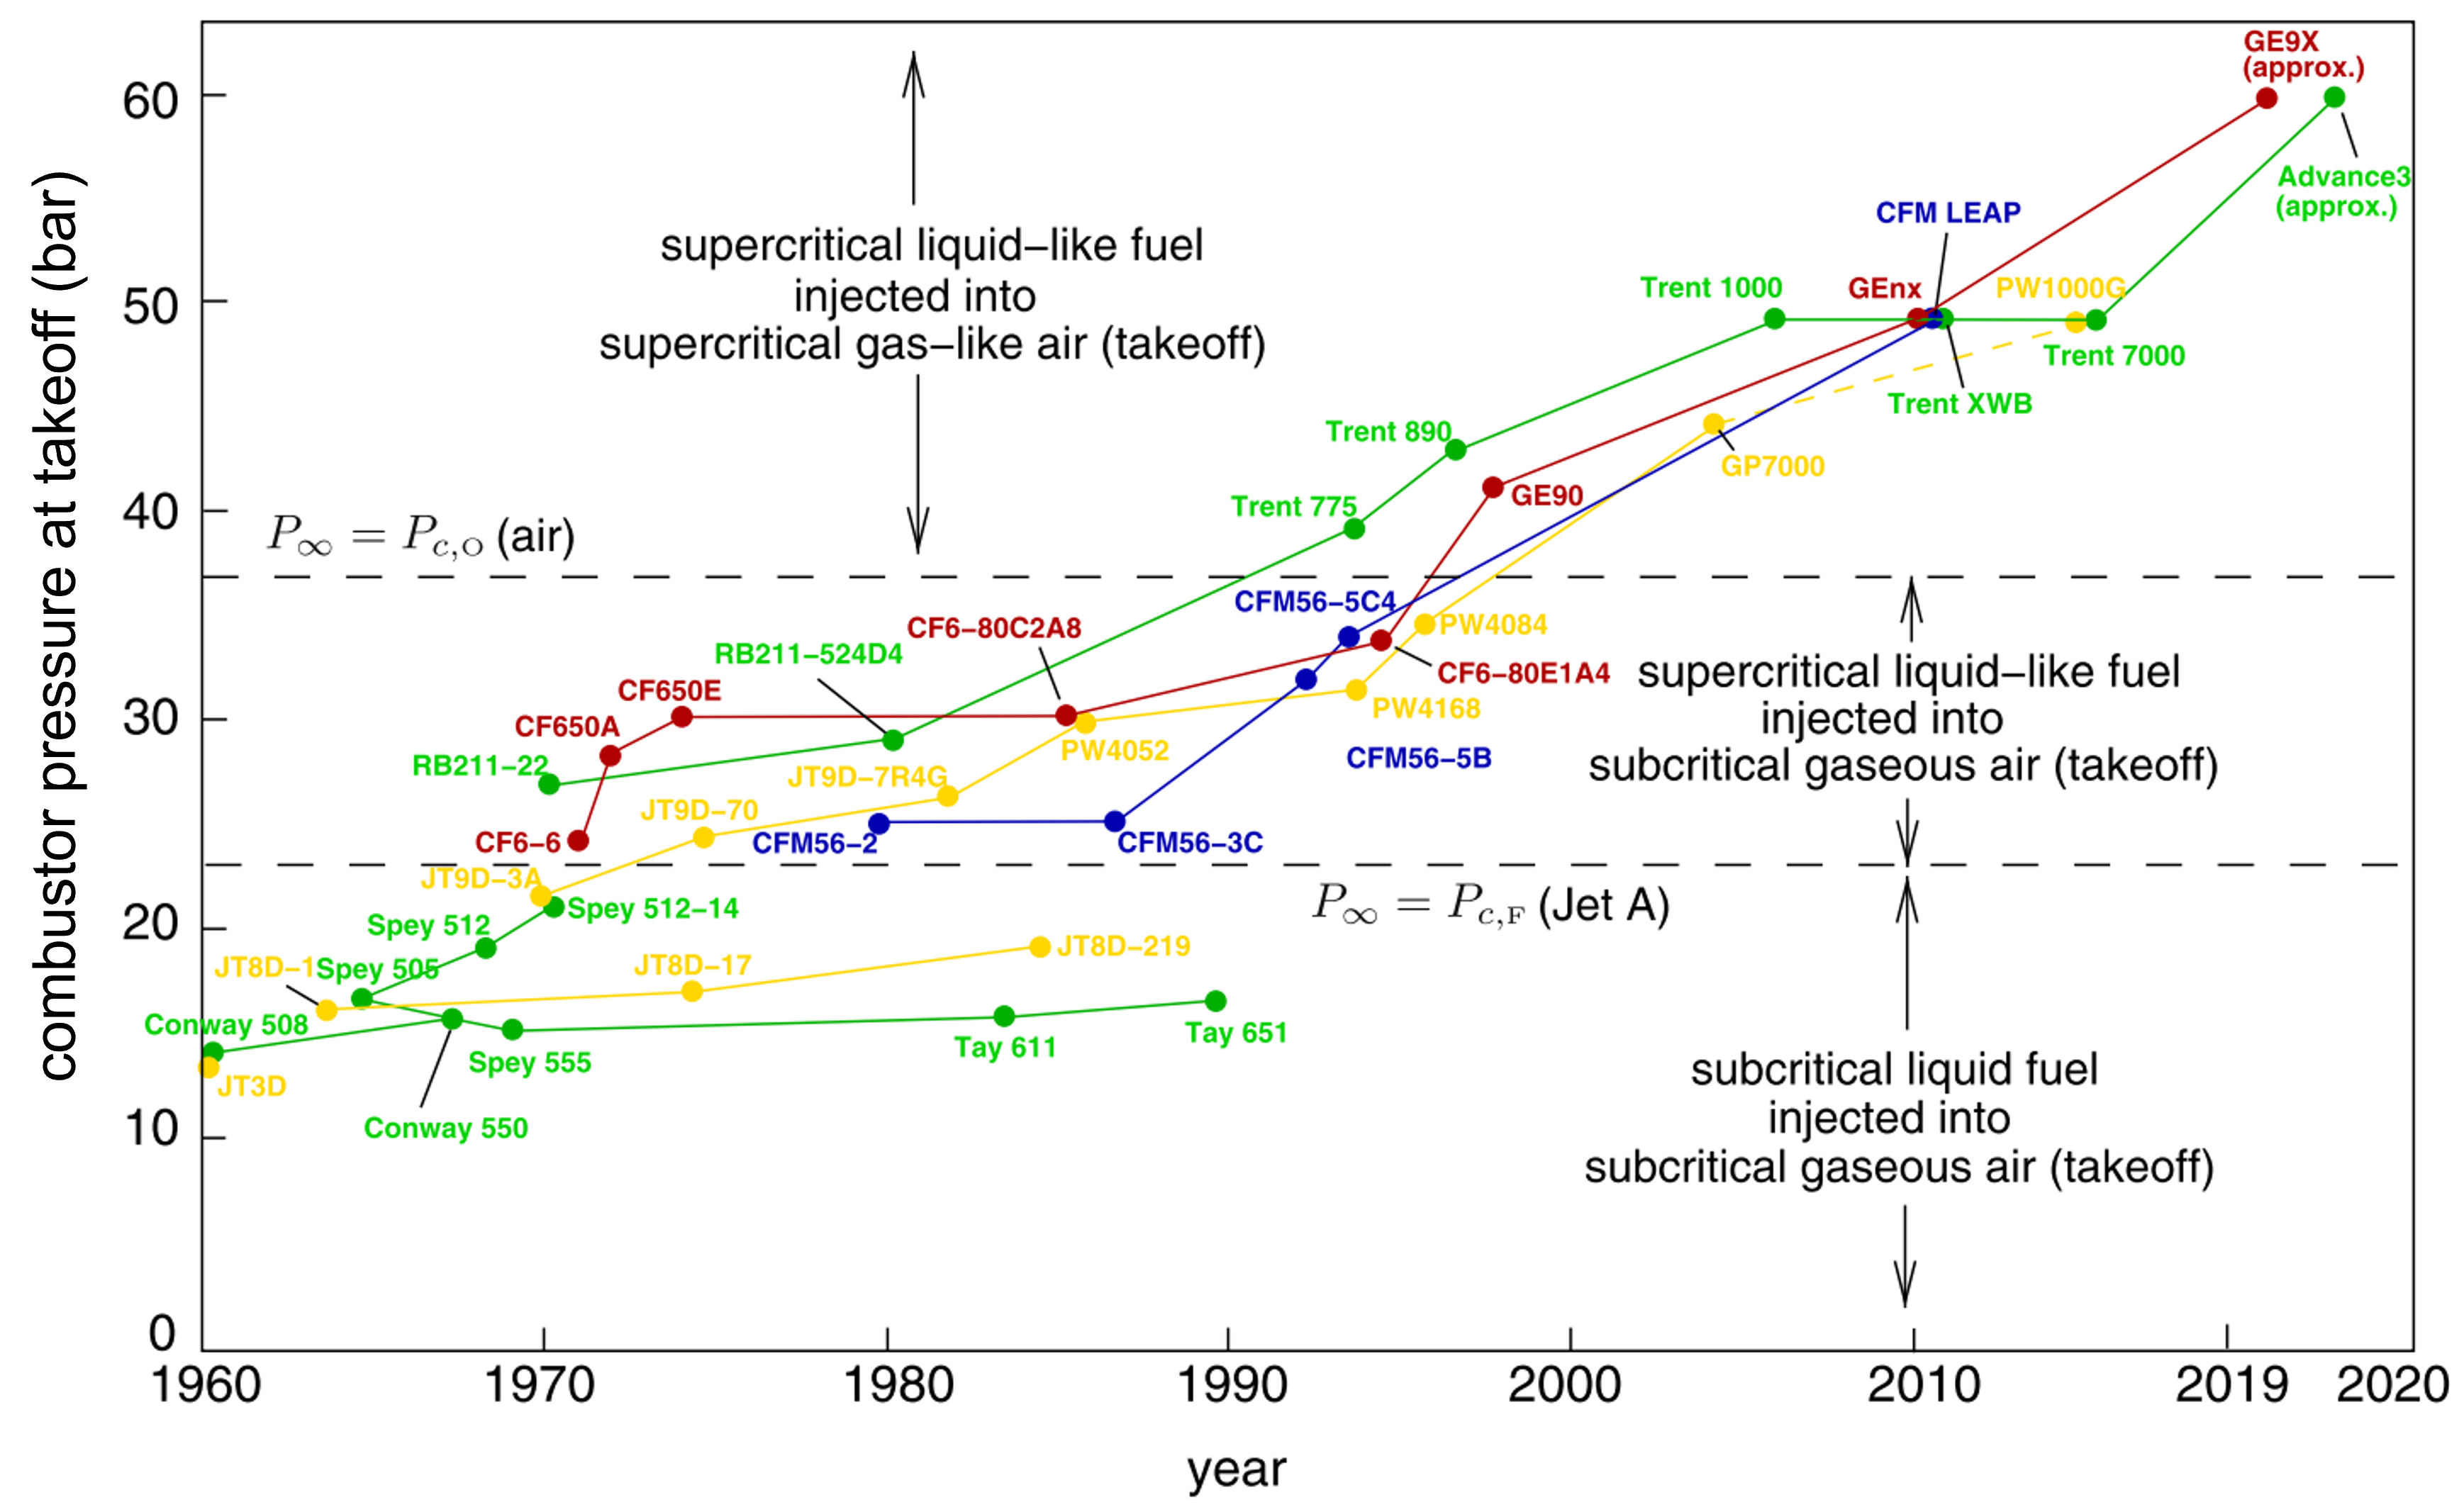
\includegraphics[width=0.95\linewidth]{gasturbine_1.png}
        %\caption{fig1}
        %\end{minipage}%
    }%
    \caption{Combustor pressure $P\infty$ in bars at sea-level takeoff for gas-turbine jet engines as a function of time (borrowed from \cite{jofre2021transcritical}). The different colors indicate manufacturers, including Rolls Royce (green), General Electric (red), CFM (blue), and Pratt \& Whitney (yellow). The upper and lower dashed horizontal lines mark the critical pressure of air ($P_{c,O}$ = 36 bar) and Jet-A ($P_{c,F}$ = 24 bar).} \label{Intro_gas_turbine}. 
\end{figure}


%%Consequently, transcritical/supercritical effects are introduced into the combustion system, causing a complete change in the underlying physics when compared to subcritical systems. The term \textbf{transcritical} in this work refers to an operating pressure higher than the critical pressure of the pure fuel or oxidizer while remaining below the cricondenbar pressures of their possible mixtures \cite{fathi2022large}. As a result, the transcritical flow may involve phase separation. On the other hand, the term \textbf{supercritical} fluid refers to an operating pressure higher than the cricondenbar pressures, where phase separation can not occur, but strong non-ideal effects can still be observed. Since the critical pressure of the mixture is often higher than the critical pressure of the each component, many nominally supercritical system may still be transcritical. Fig~\ref{Intro_critical_loci} presents the phase diagrams of Type I and Type III mixtures showing their phase separation behaviors. The mixture classification scheme is from van Konynenburg and Scott \cite{van1980critical}. 

%%For Type I mixture, one critical curve connects the critical point of the two pure component. However, For Type III mixtures, two distinct critical curves are present, one starting from the critical point  of the component with relatively higher critical temperature, and goes to infinite pressures; the other one starts at the critical point of the component with lower critical temperature and ends at the upper critical point intersecting with the three-phase vapor-liquid-liquid coexistence line. Hence, Phase separation may happen for Type III mixtures even at very high pressures. Most of the binary mixtures of nitrogen and hydrocarbons exhibit Type III phase behavior. Hence, Type III mixtures are of more relevance to propulsion systems, most high-pressure combustion systems are transcritical in practice.  


As a consequence, the introduction of transcritical/supercritical effects into the combustion system brings about a profound transformation in the underlying physics when contrasted with subcritical systems. In this context, the term \textbf{transcritical} is employed to denote operating pressures that exceed the critical pressure of the pure fuel or oxidizer while remaining below the cricondenbar pressures of their possible mixtures \cite{fathi2022large}. Consequently, transcritical flow scenarios may encompass phase separation phenomena. In contrast, the term \textbf{supercritical fluid} signifies operating pressures surpassing the cricondenbar pressures, where phase separation becomes improbable, yet strong non-ideal effects remain observable. Since the critical pressure of a mixture often exceeds that of its individual components, many nominally supercritical systems may, in fact, exhibit transcritical behavior. Illustrated in Fig.~\ref{Intro_critical_loci} are phase diagrams for Type I and Type III mixtures, delineating their distinct phase separation characteristics. This classification system for mixtures adheres to the framework developed by van Konynenburg and Scott \cite{van1980critical}.

In the case of Type I mixtures, a single critical curve connects the critical points of the two pure components. However, for Type III mixtures, a distinct dual-critical curve phenomenon emerges. One originates from the critical point of the component possessing the relatively higher critical temperature, extending to infinite pressures. The other commences at the critical point of the component with the lower critical temperature, and concludes at the upper critical point, intersecting with the three-phase vapor-liquid-liquid coexistence line. Consequently, Type III mixtures may undergo phase separation even under exceedingly high pressures. This behavior is particularly pertinent in the context of propulsion systems, where many binary mixtures of nitrogen and hydrocarbons exhibit Type III phase characteristics. For practical purposes, particularly in propulsion systems, it's worth noting that the majority of high-pressure combustion systems operate in transcritical regimes, emphasizing the relevance of Type III mixtures in these applications.


\begin{figure}[htb]
    \centering
    \subfigure{
        %\begin{minipage}[t]{0.5\linewidth}
        \centering
        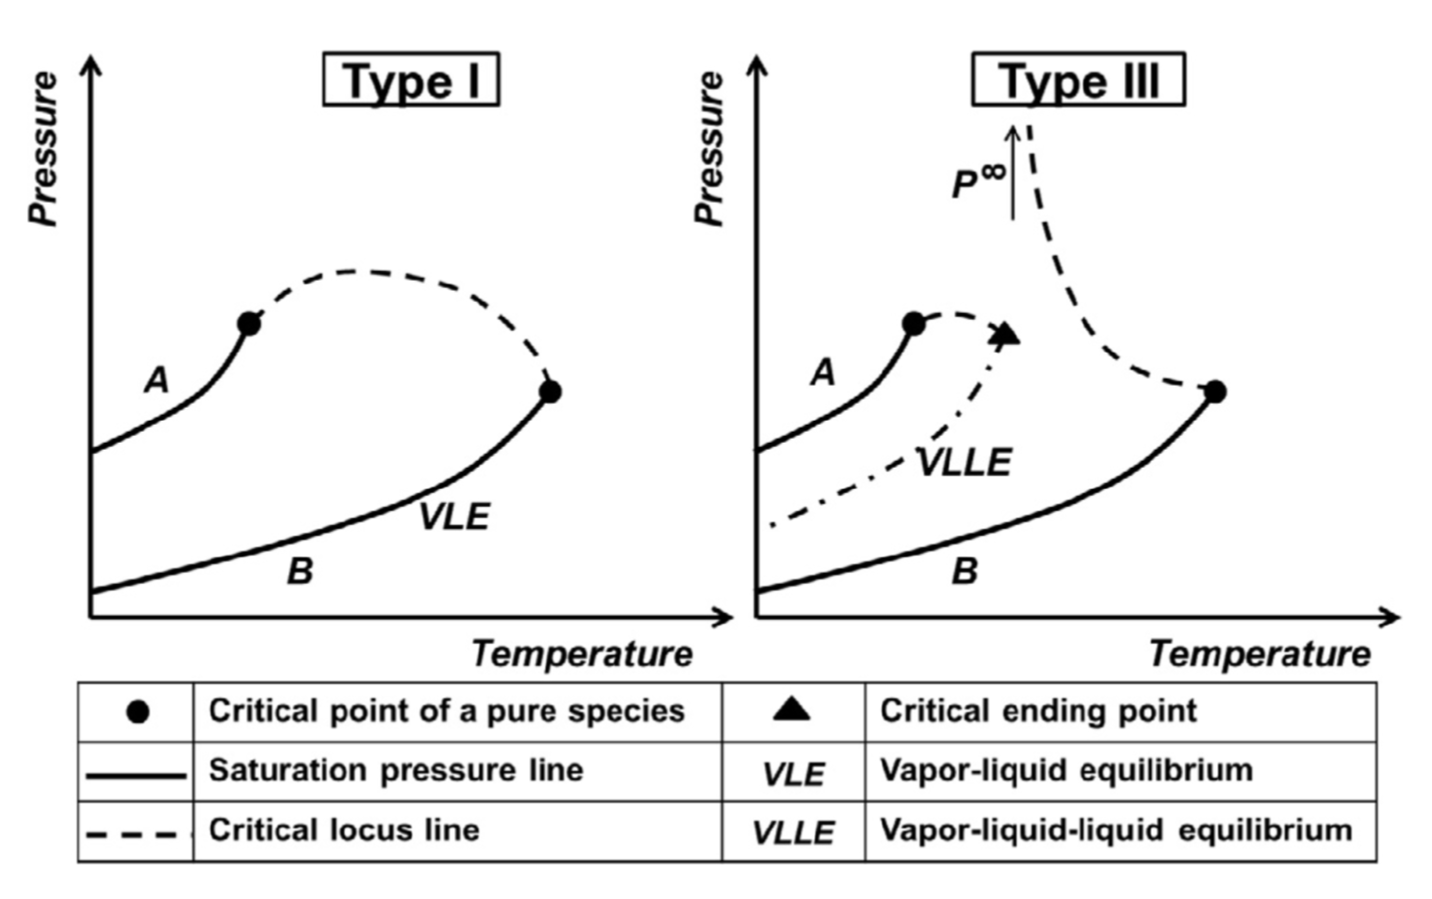
\includegraphics[width=0.95\linewidth]{critical_loci.png}
        %\caption{fig1}
        %\end{minipage}%
    }%
    \caption{Critical loci curves for Type I and Type III mixtures (borrowed from \cite{qiu2015investigation})} \label{Intro_critical_loci}. 
\end{figure}


Fig.~\ref{Intro_trans_exp} serves to illustrate the distinction between subcritical and supercritical injection scenarios. In examining the outcomes of two distinct injectors, a discernible contrast emerges: subcritical jet injection yields a clearly defined phase boundary, whereas under supercritical conditions, the interface between the pseudo phases, characterized as liquid-like and gas-like phases, becomes diffused. The phenomenon of supercritical jet breakup deviates markedly from the classical mechanisms observed at lower pressures, where surface tension exerts dominant influence. This phenomenon has garnered extensive attention in numerous experimental investigations, including both single-component \cite{mayer1998atomization,chehroudi2002visual,candel2006structure,oschwald2006injection,roy2013disintegrating} and multi-component systems \cite{mayer1998atomization,chehroudi2002visual,candel2006structure,oschwald2006injection,roy2013disintegrating}. Unlike interfaces governed by surface tension, these diffused interfaces, devoid of surface tension effects, fundamentally alter the dynamics of the jet breakup process. Instead of surface forces, diffusion emerges as the primary driving force \cite{chehroudi1999initial,smith2004fundamentals}. Within combustors, the chronological sequence of physical processes following injection adheres to a specific pattern: liquid atomization, evaporation, mixing, and chemical reactions. Atomization plays a pivotal role in facilitating complete evaporation, which can have a significant impact on cold ignition and combustion efficiency within the combustor. Consequently, a comprehensive understanding of high-pressure injection and mixing processes becomes imperative, particularly in the context of modern combustor design, which encompasses injector design considerations. However, it is important to acknowledge the formidable challenges associated with modeling both non-reacting and reacting flows at elevated pressures.


%%Fig.~\ref{Intro_trans_exp} shows the difference between subcritical and supercritical injection. In the results of two difference injectors, we can see that the subcrtical jet show clear phase boudanry, while under supercritical conditions, the interface between the pseudo phases (i.e., the liquid-like and gas-like phases) becomes diffused. Supercritical jet breakup exhibits a distinct behavior from the classical mechanism observed at low pressures, where surface tension plays a dominant role. This phenomenon has been extensively documented in many experimental studies involving both single-component \cite{mayer1998atomization,chehroudi2002visual,candel2006structure,oschwald2006injection,roy2013disintegrating} and multi-component systems \cite{mayer1998atomization,chehroudi2002visual,candel2006structure,oschwald2006injection,roy2013disintegrating}. Unlike interfaces with surface tension, the absence of surface tension in these diffused interfaces alters the dynamics of jet breakup. Instead of being dominated by surface effects, the breakup process is primarily driven by diffusion \cite{chehroudi1999initial,smith2004fundamentals}. 


\begin{figure}[htb]
    \centering
    \subfigure{
        %\begin{minipage}[t]{0.5\linewidth}
        \centering
        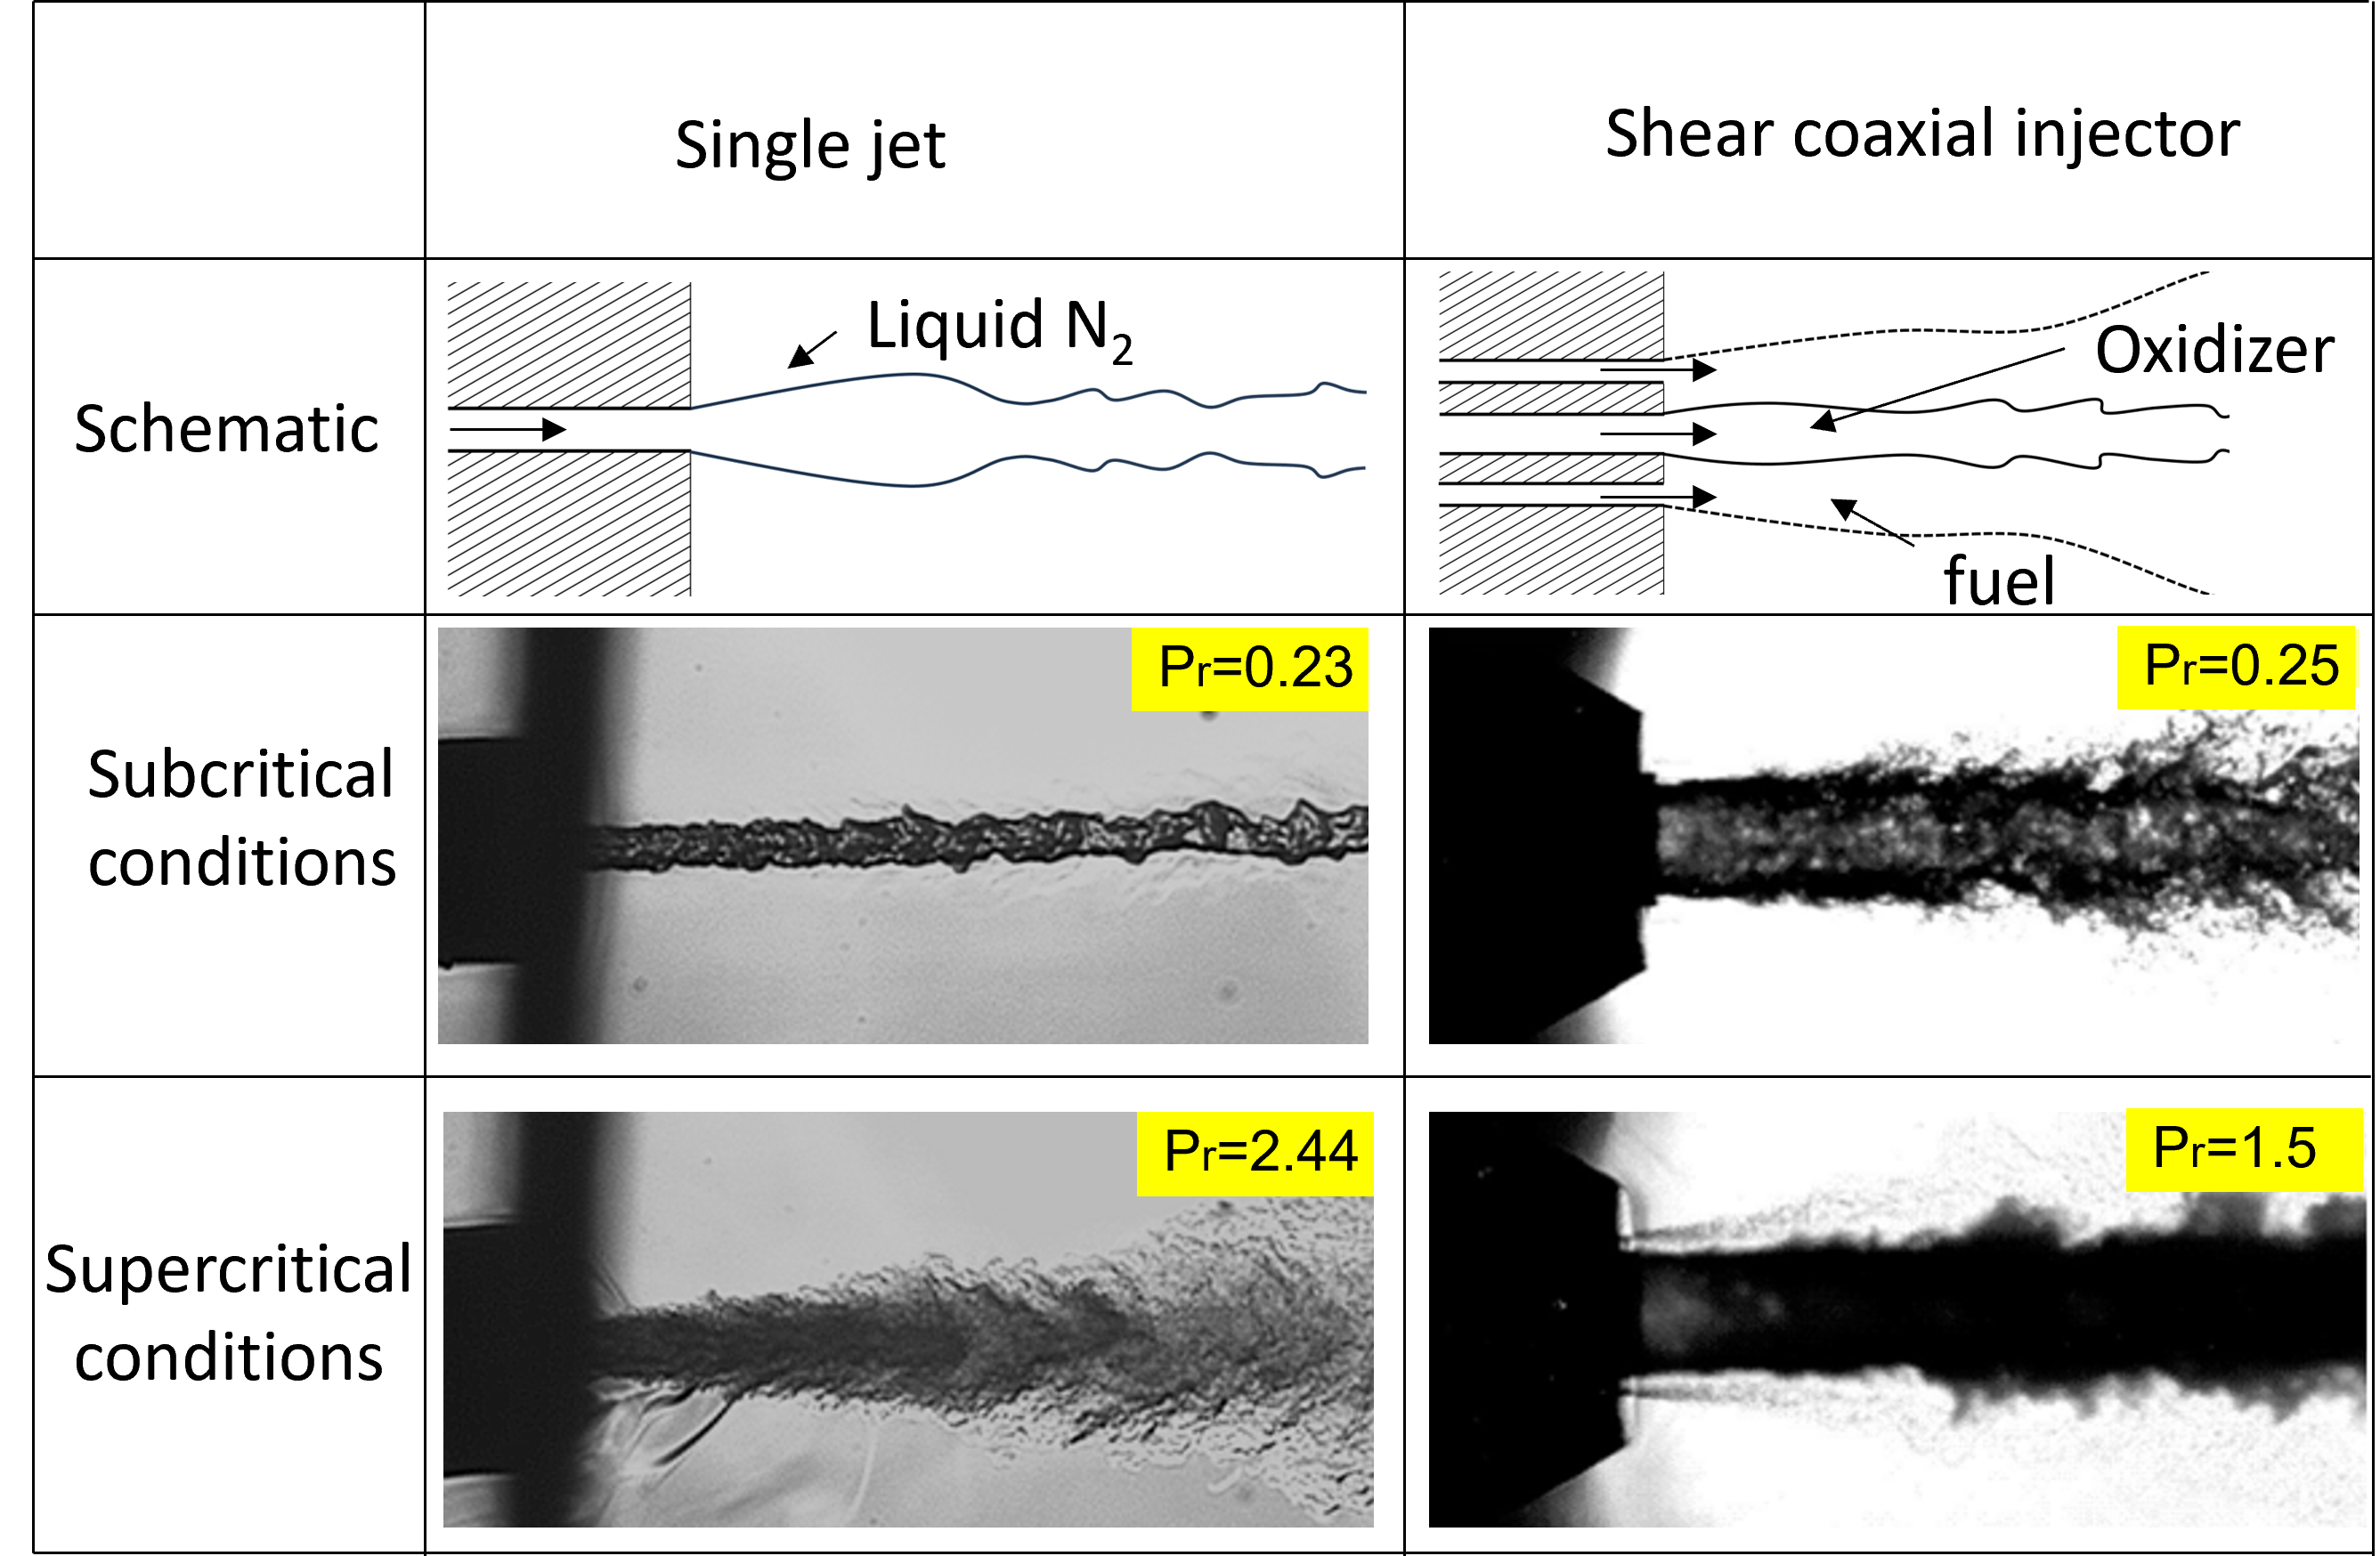
\includegraphics[width=0.95\linewidth]{trans_exp.png}
        %\caption{fig1}
        %\end{minipage}%
    }%
    \caption{Comparision bewteen subcritical injection and supercritical injection. Single jet results are from \cite{chehroudi1999initial}, and coaxial injection results are from \cite{telaar2000experimental}} \label{Intro_trans_exp}. 
\end{figure}



%%In combustors, the physical processes that occur after injection follow a specific sequence: liquid atomization, evaporation, mixing, and chemical reactions. Atomization plays a crucial role in achieving complete evaporation, which can have a significant impact on cold ignition and combustion efficiency within the combustor. As a result, it is essential to have a thorough understanding of high-pressure injection and mixing processes, particularly when designing modern combustors, including the injector design. However, there are great difficulties when attempting to model the non-reacting and reacting flows at high pressures. 

The first difficulty in modeling transcritical/supercritical flows is that at high pressure, the gaseous/gas-like fluid does not satisfy the ideal gas law, and this makes transcritical/supercritical fluid behavior peculiar because of the large variation of thermodynamic properties such as density and specific heat near the critical point. Accurately describing these properties requires the use of a real-fluid equation of state (EOS). Among the commonly employed options, cubic equations of state, such as the Peng–Robinson (PR) EOS \cite{peng1976new} and Soave–Redlich–Kwong (SRK) EOS \cite{soave1972equilibrium}, are popular choices for transcritical/supercritical flow simulations due to their computational efficiency and acceptable accuracy. Additionally, volume translation methods can be utilized to improve density prediction further \cite{muller2016large}. While more sophisticated equations of state are available, such as the Benedict–Webb–Rubin equation \cite{benedict1940empirical} and the statistical associating fluid theory (SAFT) \cite{gross2001perturbed} formulated in the Helmholtz free energy, they often come with higher computational costs and increased complexity. Implementing phase change models based on these EOS can be challenging due to their intricacy. 
Therefore, for this work, the PR EOS has been selected.

The non-ideal/real-fluid effects observed in transcritical/supercritical flows have been known to cause spurious pressure oscillations in numerical simulations that employ fully conservative (FC) schemes \cite{schmitt2010large,terashima2012approach,ruiz2012unsteady,hickey2013large,kawai2015robust}. To address this issue, several approaches have been proposed that trade off full conservation for improved stability and accuracy, leading to the development of quasi-conservative schemes. One such scheme, introduced by Schmitt et al., involves incorporating an artificial viscosity term derived from the pressure equation \cite{schmitt2010large}. By adding this term, the scheme effectively dampens pressure oscillations. Another approach, proposed by Johnson and Ham, introduces an additional transport equation for a function of the specific heat ratio \cite{johnsen2012preventing}. Lacaze et al. put forward an enthalpy-based quasi-conservative scheme, which mitigates the loss of conservation \cite{lacaze2019comparison}. Abgrall and Karni developed the double flux (DF) method \cite{abgrall2001computations}, which has been extended for reacting flows \cite{billet2003adaptive}, as well as for use with discontinuous Galerkin methods \cite{billet2011runge,lv2014discontinuous} and transcritical flows \cite{ma2017entropy,tudisco2020numerical}. The DF method \cite{ma2017entropy} is integrated into the computational fluid dynamics (CFD) solver and has demonstrated favorable behavior in handling the non-ideal effects associated with transcritical flows. In the present work, the DF method is incorporated into the CFD solver and its performance and behavior is evaluated to understand its ability to handle the challenges posed by transcritical/supercritical flows.


The second difficulty in modeling transcritical flows arises from phase change phenomena. While the operating conditions may be nominally supercritical with respect to a single component, the local mixture can remain in the subcritical two-phase regime. This occurs because the critical pressure of the mixture can be significantly higher than the critical pressure of each individual component forming the mixture \cite{van1980critical,tudisco2020numerical,zhang2022multicomponent}. Hence, most multi-component transcritical systems exhibit a hybrid behavior, with a subcritical two-phase interface (involving phase change) and a supercritical diffused mixing layer (without phase change) coexisting at different locations. %This hybrid behavior will also be discussed in Sec.~\ref{sec:result} of the present paper. 
Although there has been considerable interest in modeling transcritical/supercritical injection and mixing over the past three decades, most studies have struggled to capture this hybrid behavior effectively. Some researchers have used Lagrangian particles to track droplets \cite{pei2015large,kahila2018large,gadalla2020large}, but the breakup and evaporation processes of the droplets were empirically modeled using sensitive tuning parameters. The tuning of these parameters heavily relies on the availability of experimental data. Another approach is the dense-fluid method \cite{yang2000modeling,lacaze2015analysis,jofre2021transcritical}, which accounts for the real-fluid effects but neglects phase boundaries and phase change since it assumes that the entire system is within the supercritical single-phase regime. 


To overcome the limitations of these methods, a two-phase diffuse-interface method based on vapor-liquid equilibrium (VLE) theory has been introduced. In this method, the fully compressible Navier–Stokes equations are solved to obtain local mixture properties such as density, internal energy, and component mass fraction. These properties are then used as inputs to compute other thermodynamic and transport properties using the VLE theory, which is based on a real-fluid equation of state. The VLE theory is derived from the principle of minimizing the Gibbs free energy and accurately describes multiphase flow physics, including high-pressure phase change, preferential evaporation, and gas dissolution in the liquid phase. The VLE-based two-phase diffuse-interface method has been successfully applied to simulations involving ECN Spray A \cite{matheis2018multi, yang2020real}, flash boiling \cite{yi2019multicomponent}, %supercritical \ce{CO2} systems \cite{zhang2022multicomponent},
cavitation \cite{yang2020parametric}, mixing layers \cite{tudisco2020vapor}, and reacting flows \cite{fathi2022large,srinivasan2023vle}. It offers a promising approach for capturing the complex behavior of transcritical flows with phase change and has shown good agreement with experimental observations. 


However, the computational cost of vapor-liquid equilibrium (VLE) calculations can be prohibitively high \cite{yi2019numerical,yang2020real}%,zhang2022multicomponent},
,particularly when dealing with a large number of components or a large computational domain. To address this issue, researchers have developed tabulation approaches that aim to accelerate thermodynamic model computation.
 
One such approach is the tabulated thermodynamic model based on the NIST REFPROP database and VLE with the Peng–Robinson (PR) equation of state (EOS) proposed by Koukouvinis et al \cite{koukouvinis2020high}. This method stores the thermodynamic properties in a structured table in log10(p)-T form, enabling efficient lookup during the simulation.
Additionally, an efficient tabulation approach for binary mixtures, which supports reverse look-up using the inverse-distance weighting method, has been developed for VLE calculations of binary mixtures \cite{yi2019numerical,jafari2021towards,jafari2022exploring}. This approach has been successfully employed in investigating transcritical droplet injection. Furthermore, the tabulation method has been extended to ternary mixtures to study droplet evaporation \cite{gaballa2022numerical}. %We also developed a tabulation method based on Ping et al.'s work \cite{yi2019numerical} to investigate phase separation in supercritical \ce{CO2} systems \cite{zhang2022multicomponent}. 
These tabulation methods offer computationally efficient and robust VLE solutions for CFD simulations. However, it's important to note that the memory requirement of tabulation methods grows exponentially with the number of components, leading to unaffordable memory demands for larger systems (i.e., the curse of dimensionality: table size $\sim M^N$, where $M$ is the number of grids of each component in the table and $N$ is the number of components). %For example, using a table with the same resolution as mentioned in our previous work (e.g., a table with variable range: $T$ 470-600 K, $P$ 9-25 MPa, $x_i$ 0.6-0.9, and interval: $\Delta T = 1.3$ K, $\Delta P = 0.4$ MPa, $\Delta x_i = 0.015$) \cite{zhang2022multicomponent} for a 4-component system, would result in a table size of approximately 4 terabytes (TBs). 
Storing such large tables in each CPU core (without shared memory) or each node (with shared memory) becomes infeasible for existing computing facilities. Consequently, these traditional tabulation methods are typically limited to binary or at most ternary systems and are unsuitable for multiphase combustion and other multi-component problems. Recently, artificial neural networks (ANNs) have emerged as an alternative to tabulation methods and have been proposed as nonlinear regression models for thermodynamic properties \cite{wang2019accelerating,koukouvinis2022machine}. ANNs offer the advantage of easier extension to a large number of components, mitigating the curse of dimensionality associated with tabulation methods. However, controlling the error and ensuring accurate performance of ANNs can be challenging, as their accuracy heavily relies on the training process.


%A paragraph about ISAT method (TODO)

As an alternative to the conventional tabulation method, the \textit{In Situ} Adaptive Tabulation (ISAT) \cite{pope1997computationally} approach has been gaining increasing attention. ISAT is an on-the-fly tabulation method, based on multiple linear regressions that are dynamically added as additional information is discovered. Initially designed to expedite combustion chemistry calculations, ISAT achieved a remarkable 300-fold speedup ratio in the computation of the Homogeneous Charge Compression Ignition (HCCI) process \cite{contino2011coupling}, and an impressive 1000-fold speedup ratio in the calculation of the Premixed Pairwise Mixing Stirred Reactor (PPMSR) \cite{yang1998treating}. ISAT has demonstrated its adaptability across diverse problem domains, encompassing areas such as chemical engineering \cite{shah1999computational,kolhapure2005pdf,10.1115/1.2709655}, surface reactions \cite{mazumder2005adaptation}, thin film growth \cite{varshney2005multiscale}, solid mechanics \cite{arsenlis2006generalized}, control systems \cite{hedengren2008approximate}, and turbulent combustion models based on manifolds \cite{lacey2021situ}.

One of ISAT's key advantages is its ability to construct tabulations on-the-fly, minimizing memory requirements and effectively combating the curse of dimensionality by storing only essential data. Moreover, ISAT achieves computational efficiency on par with traditional tabulation methods while bypassing the need for time-consuming pre-processing steps like table generation or neural network training. Computation occurs in real-time, eliminating the necessity for extensive setup procedures.

ISAT maintains precise error control by defining finer granularity in regions exhibiting heightened nonlinearity. Furthermore, the degree of error control in ISAT can be adjusted to meet specific accuracy requirements, offering superior flexibility compared to traditional tabulation and artificial neural networks (ANN). Consequently, ISAT stands as an exceedingly efficient acceleration method suitable for thermodynamic models, such as VLE models.

%%In this work, we developed a novel method for accelerating VLE-based CFD simulations by employing \textit{In Situ} Adaptive Tabulation (ISAT) \cite{pope1997computationally}. Originally designed to expedite combustion chemistry calculations, ISAT has proven to be adaptable to various problem domains, including chemical engineering \cite{shah1999computational,kolhapure2005pdf,10.1115/1.2709655}, surface reactions \cite{mazumder2005adaptation}, thin film growth \cite{varshney2005multiscale}, solid mechanics \cite{arsenlis2006generalized}, control systems \cite{hedengren2008approximate}, and turbulent combustion models based on manifolds \cite{lacey2021situ}. By constructing the tabulation on-the-fly, ISAT minimizes memory requirements and effectively addresses the curse of dimensionality by storing only essential data. Moreover, it achieves computational efficiency comparable to traditional tabulation methods. Unlike other approaches, our proposed ISAT-VLE method does not necessitate pre-processing steps such as table generation or neural network training. Computation is performed in real-time, eliminating the need for extensive setup procedures. This method is integrated with a CFD solver based on the central-upwind scheme \cite{kurganov2000new,greenshields2010implementation}, enabling the simulation of multiphase transcritical flows. To evaluate the performance and error control of our model, we conducted transcritical temporal mixing layer and shock-droplet interaction simulations. Phase separation is captured in both simulations. In the shock-droplet interaction simulations, we compared the performance and error control of ISAT of the DF scheme with those of the FC scheme and evaluated the DF's spurious oscillation removal. 

\section{Objectives}

our obajecttivs are creasting new devedlope a transcritical VLE model 

anayliyze scO2 system 

deveop a ISAT -VLE modle 

develope shared memoty ISAT model


\section{Outline of the Thesis}





%%%%%%%%%%%%%%%%%%%%%%%%%%%%%%%%%%%%%%%%%%%%%%%%%%%%%%%%%%%%%%%%%%%%%%%%%%%%%%%%
